\chapter{Introduction}
\label{Chapter1}
\settocdepth{subsection}
Image edge detection and image segmentation are key problems in computer vision.
%While the two problems are related

\section{Motivation}
Recently, very good edge detection results were achieved using random decision forests \cite{DollarICCV13edges}. While a certain edge model is imperative, % required, needed % a requirement
few segmentation algorithms use edge detection output as a first step to image segmentation. Consequently, many edge detection algorithms re-use the same approach to obtain image segmentation in addition %additionally 
to their edge detection output.

Therefore, the field is limited by lack of research on the problem of edge-based hierarchical segmentation. We investigate an alternative way % possibility 
to obtain image segmentation, given an edge detector output.

\section{Problem definition}
% TODO talk about ``semantic'' segmentation. Semantic segmentation means that the segments discovered are meaningful in a higher-level sense - they are objects, or prominent part of objects. Therefore the regions in the segmentation should respect %
% not cross boundaries of objects.

We address the problem of semantic image segmentation. To help understand it, it is necessary to first introduce the notions of an {\it edge} - an essential for edge detection, and {\it contour} - a prerequisite for image segmentation.

\textbf{Terminology:} As the field is young, it is worth pointing out that there is a certain lack of consistency and differences in definitions as concerns related terminology. In the following we define the basic vocabulary for our method and we will be consistent in using it throughout this report.

\subsection{Edge detection}
The detection of edges in digital images has its application in %tasks such as 
object detection and recognition, segmentation, structure from motion, and tracking.

% TODO use a horizontal image as example, will fit two at a line without taking so much space
\begin{figure}[ht!]
\centering
 \subfigure[Input image from %the validation subset of 
 BSDS500~\cite{BSDS500resources}]{%
  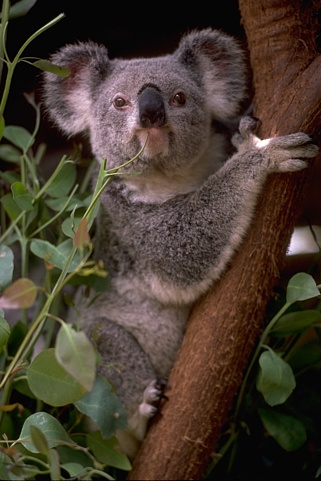
\includegraphics[width=0.35\textwidth]{images/examples/koala/koala.jpg} % hawaii/arbelaez2011-035.png}
 }
 \subfigure[Edge map]{%
  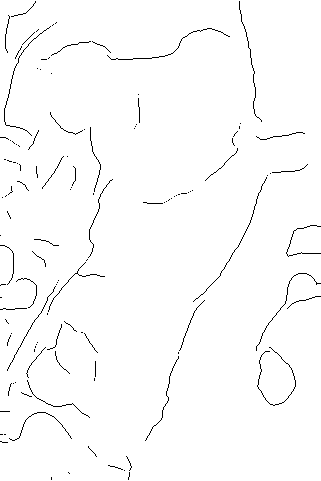
\includegraphics[width=0.35\textwidth,frame]{images/examples/koala/koala_gPb_edge_map.png} % too thin - SE are thicker koala_SE_edge_map % hawaii/edge_map_arbelaez2011-039.png}
  \label{fig:sub:edge_detection-edge-map}
 }

 \subfigure[Probability of boundary ({\bf Pb})]{%
  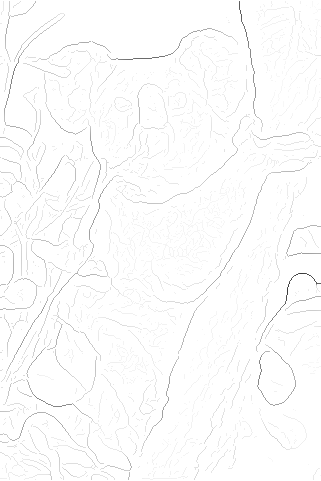
\includegraphics[width=0.35\textwidth,frame]{images/examples/koala/koala_gPb.png} % koala_SE % hawaii/Pb_arbelaez2011-039.png}
  \label{fig:sub:edge_detection-pb}
 }
 \subfigure[{\bf Pb}, jet colour-coded]{%
  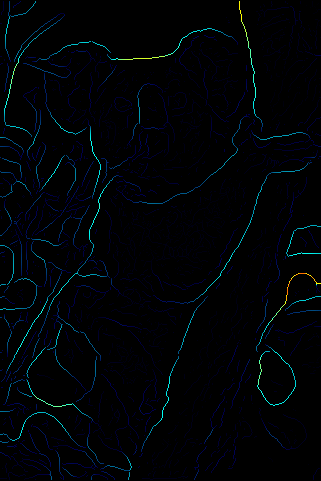
\includegraphics[width=0.35\textwidth]{images/examples/koala/koala_gPb_cc.png} % koala_SE_cc % hawaii/Pb_arbelaez2011-039.png}
  \label{fig:sub:edge_detection-pb-cc}
 }
\caption[Edge detection - edge map and probability of boundary]{{\bf Edge detection}. Note that for ease of view, %illustration
the negative of \protect\subref{fig:sub:edge_detection-edge-map} and \protect\subref{fig:sub:edge_detection-pb} are shown, \ie the darker the pixel, the higher the probability of an edge. Visualisation code for \protect\subref{fig:sub:edge_detection-pb-cc} courtesy of Hallman and Fowlkes~\cite{Hallman2014}.}
\label{fig:edge_detection}
\end{figure}

\subsubsection{Edge, edge map, probability of boundary}
\textbf{Image edge:} Image edge detection deals with the problem of finding pixels which belong to object boundaries within a digital image. The pixels belonging to object boundaries in an image are often locations where a sharp change of image brightness occurs. Those locations of image intensity discontinuities are called \textit{image edges}. In photographs edge pixels are grouped together due to the properties of natural images.

\textbf{Edge map:} We will call an \textit{edge map} a binary image $M$ depicting edges locations. The pixels belonging to an edge are set to 1. The rest of the pixels are not part of an edge. They have a value of 0. Therefore, for a given pixel location $(x,y)$, the corresponding edge map value is $M_{(x,y)} \in \{0,1\}$ (see \fref{fig:sub:edge_detection-edge-map}).

\textbf{Probability of boundary:} To allow to express a level of (un)certainty as to the presence of an edge in an image, we employ a probabilistic means. We define a real-valued image $Pb$, which stands for \textit{Probability of boundary} (see \fref{fig:sub:edge_detection-pb} and \fref{fig:sub:edge_detection-pb-cc}). For a given pixel location $(x,y)$, the corresponding value is $Pb_{(x,y)} \in [0,1]$.

The notion of probability of a location being an edge pixel was first introduced in~\cite{martin2004learning}. % TODO really?
It has ever since been used as an output to many edge detection algorithms~\cite{Maire2008using,LimZD13,DollarICCV13edges,Isola2014crisp,Ganin2014n4fields,Hallman2014}.

\textbf{Thresholding:} Given a Pb, we can obtain edge maps at different levels of detail by {\it thresholding}. We choose a threshold $t\in(0,1)$ and consider as detected edge pixels those locations $(x,y)$ for which it holds %such that 
$Pb(x,y)>t$. Obviously, a lower threshold allows to discover more edges, while a higher threshold is more conservative and would only honour the most salient of edges.

\textbf{Example:} In \fref{fig:edge_detection} we show the result of the edge detection algorithm gPb~\cite{Arbelaez11}.

The last two images visualise the detector output - a {\it Probability of boundary} ({\bf Pb}). For improved viewing in case of probabilistic output we will utilise a visualisation with black as background and heatmap-coloured boundaries according to their strength. This visualisation of probabilistic output facilitates the qualitative comparison of the results of different algorithms. 

The edge map \fref{fig:sub:edge_detection-edge-map} was obtained by thresholding at $t=0.3$ the {\it Pb} \fref{fig:sub:edge_detection-pb}.

%- TODO general consensus in the community that edge detection is somewhat ill defined in that it is not quiteclear what defines a correct output \cite{martin2004learning}

\subsection{Image segmentation}
Segmentation is the task of partitioning a digital image into meaningful parts. Those parts, called segments, should unify homogenous regions. The purpose of this decomposition is to ease further analysis by substituting reasoning on the \textit{\textbf{superpixels}} (another term for the segments) {\it graph} for reasoning on the {\it pixels grid}. % substitute sth for sth: ``Industry must reduce fuel consumption by substituting alternative fuels for fossil fuels.''


% TODO: for image segmentation 
% If the task is unspecified as a general video segmentation task, then there is an ambiguity of the correct level of granularity on the ground truth segments, and different human annotators would show different acceptable ways to segment the video. And one can see the agreement among the human annotators are around 80-90 percent. Especially, they tend to agree on the main subjects but differ on the background ones.
%
% from \cite{Martin01}:
% It is imperative that variation among human segmenta-tions of an image is due to different perceptual organiza-tions of the scene, rather than aspects of the experimentalsetup. In order to minimize variation due to different inter-pretations of the task, the instructions were made intention-ally vague in an effort to cause the subjects to break up thescene in a ``natural'' manner:Divide each image into pieces,where each piece represents a distinguished thing in the im-age. It isimportant that all of the pieces have approximatelyequal importance. The number of things in each image is upto you.  Something between 2 and 20 should be reasonablefor any of our images.

\begin{figure}[ht]
\centering
 \subfigure[Input image]{%
  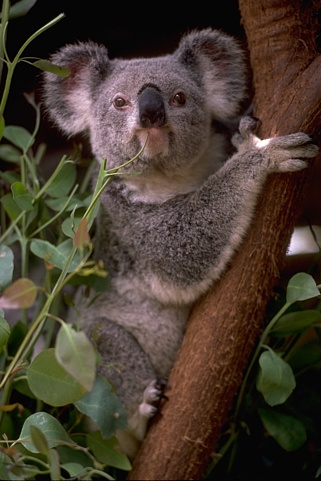
\includegraphics[width=0.1\textwidth]{images/examples/koala/koala.jpg}
 }
 \subfigure[Segmentation - labelling]{ % (implicit boundary)]{%
  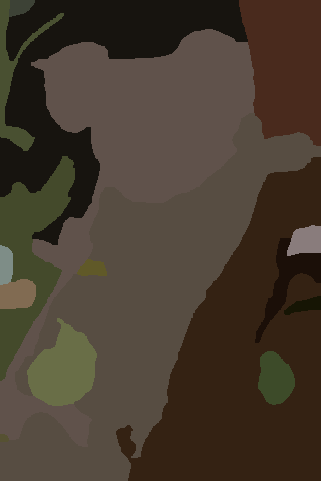
\includegraphics[width=0.2\textwidth]{images/examples/koala/koala_segm_labelling.png}
  \label{fig:sub:segmentation-segm-labelling}
 }
 \subfigure[Segmentation contours]{%
  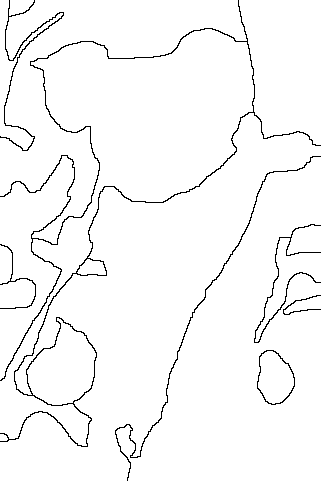
\includegraphics[width=0.2\textwidth,frame]{images/examples/koala/koala_segm_bdry.png}
  \label{fig:sub:segmentation-segm-bdry}
 }
 \subfigure[Region]{ %, segment, superpixel
  
\includegraphics[width=0.2\textwidth,frame]{images/examples/koala/koala_gPb_region.png}
  \label{fig:sub:segmentation-region}
 }
 \subfigure[Region boundary - a {\bf contour}]{%
  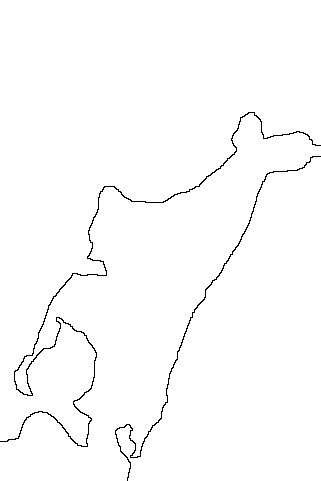
\includegraphics[width=0.2\textwidth,frame]{images/examples/koala/koala_gPb_region_bdry.png}
  \label{fig:sub:segmentation-region-contour}
 }
  \subfigure[Segmentation - explicit boundary]{%
  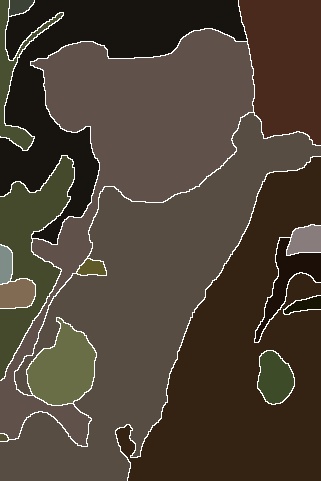
\includegraphics[width=0.2\textwidth]{images/examples/koala/koala_segm_explicit.png}
  \label{fig:sub:segmentation-segm-explicit}
 }
 \subfigure[Hierarchical segmentation - UCM~\cite{Arbelaez2006boundary}]{%
  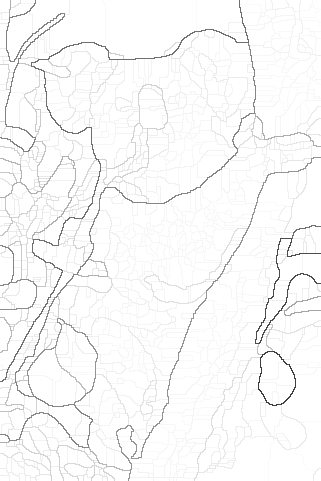
\includegraphics[width=0.35\textwidth,frame]{images/examples/koala/koala_ucm.png}
  \label{fig:sub:segmentation-ucm}
 }
 \subfigure[UCM, jet colour-coded]{%
  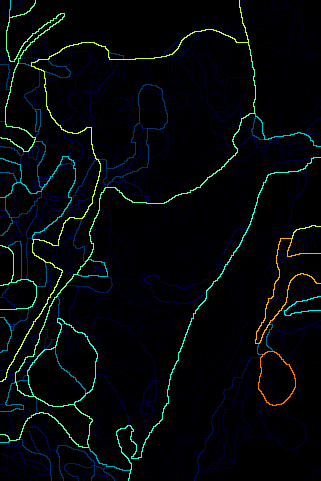
\includegraphics[width=0.35\textwidth]{images/examples/koala/koala_ucm_cc.png}
  \label{fig:sub:segmentation-ucm-cc}
 }
\caption[Image segmentation - segmentaton, contour, region, hierarchical segmentation]{{\bf Image segmentaton}. As in \fref{fig:edge_detection}, we show the negative of the probabilistic output. For segmentations we use the mean colour of the image to represent a segment. The UCMs are given larger to allow to see details.}
\label{fig:segmentation}
\end{figure}

\subsubsection{Contour, segmentation, region boundary, hierarchical segmentation}
\textbf{Image segmentation:} As already mentioned, a {\it segmentation} of a digital image is a partition of it into a set of distinct {\it segments} (also known as {\it regions}, or {\it superpixels}). In practice, we will call {\it segmentation labelling} a labelling of each pixel in the image, such that two pixels have the same label iff they belong to the same region. No two regions should have the same label. Uniqueness of segmentations is defined up to a permutation of the labels. In a segmentation we will visualise each region by its {\bf mean colour} (from the original image), as in \fref{fig:sub:segmentation-segm-labelling}.

\textbf{Region:} Regions (also {\it segments}, or {\it superpixels}) are the building blocks of a segmentation. The outline %boundary 
of a region fulfils the definition for an {\it image edge}. What is more, it constitutes a {\bf closed boundary}, which we will call {\bf contour}. See \fref{fig:sub:segmentation-region} and \fref{fig:sub:segmentation-region-contour}.

\textbf{Segmentation contours:} Note that it is {\it sufficiently easy} (further explanation to be given shortly) to obtain an {\bf edge map} from a segmentation - one just has to consider all the outlines of all the regions % superpixels
(the boundaries between the segments). The resulting edge map (\fref{fig:sub:segmentation-segm-bdry}) has the added benefit that all edges are in fact closed - they are {\it contours}.

\textbf{Segmentation represented with explicit contours:} So it is plain to see that there exists a {\bf duality between segmentation regions and contours}, in that the superpixels enclosed by the contours do %would 
form segmentation regions. If we think of the task of manually annotating a segmentation of an image, we will notice that hand-drawing the contours delineating the objects is easier than hand-labelling each pixel based on its region membership. It is more natural, therefore, to first mark %have 
the segmentation countours, and have them determine the regions - see \fref{fig:sub:segmentation-segm-explicit} for an example. In this case obtaining the segmentation contours is trivial - we just take the explicit region boundaries (and mark the pixels internal to the regions as ``background'', with an edge map value of 0), see \fref{fig:sub:segmentation-segm-bdry}.

\textbf{Segmentation contours from segmentation labelling:} In case of segmentation represented by labelling, \ie implicit boundary between regions, care must be taken in order to obtain the contours. The trouble lies in the fact that there is an ambiguity as to the correct placement of the boundaries (for a contours image with the same resolution). A possible solution is the use of {\it super-resolution}, which means doubling the resolution of the image and placing the boundaries in between the segment labels. Other solutions that don't change the image %stay on the same 
resolution should be consistent in the how exactly they place the %placement of 
boundaries when converting between the two representations.

In the rest of this report we will make use of both representations for segmentation - labelling and explicit boundaries.

\textbf{Hierarchical segmentation:} It is convenient to have a means, that in a similar way to the {\it Pb} for the task of edge detection, allows to express a degree of (un)certainty for the problem of image segmentation. Additionally, we would like to be able to obtain segmentations at different level of detail - on the full scale from an oversegmentation to an undersegmentation. That is easily possible by using a datastructure called {\it Ultrametric contour map} (UCM)~\cite{Arbelaez2006boundary}. While details will be given in \sref{sec:ch3-UCM}, for now it is sufficient to know that it encapsulates a hierarchy of segmentations. 
Like with {\it Pb}, thresholding the UCM allows to obtain a segmentation.

\textbf{Example:} In \fref{fig:segmentation} we show the result of the algorithm gPb-OWT-UCM~\cite{Arbelaez11}. The output is a UCM - see \fref{fig:sub:segmentation-ucm} for an example of UCM output and \fref{fig:sub:segmentation-ucm-cc} for its jet colour-coded visualisation.

The segmentations in % TODO
were obtained by thresholding the UCM at $t=0.4$.

\section{Related work}
%\subsection{From edges to contours}
\subsection{Edge detection}
Early edge detection approaches solely rely on local cues. Low-level detectors define edges as sharp discontinuities in image brightness. First results were achieved using digital image processing techniques. The Roberts cross~\cite{roberts1963machine}, Sobel filter~\cite{sobel19683x3}, and Prewitt operator~\cite{prewitt1970object} all are discrete differentiation operators. % can say 'differential operator'
They view an images as a 2-dimensional signal which they convolve with pre-defined filters with local support. In the same line of work is the Marr-Hildreth algorithm~\cite{marr1980theory}, which finds zero-crossings of the Laplacian of the image intensity. Later still, the Canny detector~\cite{canny1986computational} shows better-quality edges. It searches for peak gradient magnitude in the image intensity. It adds some improvements, like non-maximum suppression (also known as ``edge thinning''), which improves edge localisation. A practically relevant extensions of it is the Canny-Deriche detector~\cite{deriche1987using}, which addresses the filter implementation.

More higher-level detectors incorporate colour and texture~\cite{rubner1996coalescing,will2000learning} information, as well as multiple scales and orientations.

Globalisation-based methods.

Higher quality edge detection is desirable. Texture edges and illusory contours are ellusive to % escape from
traditional edge-detection approaches. Recent approaches therefore rely on learning to incorporate context and object knowledge. They address more challenging scenarios which arise in natural images. As Martin \etal argue in~\cite{martin2004learning}, those methods solve the so-called ``boundary detection'' problem. A boundary delineates the pixels that belong to one object, material, or surface from those that belong to another. One possible approach to boundary detection would be to use edges as low-level cues to judge for the presence of object boundaries (a bottom-up approach). Another solution is to go top-down and use higher-level object knowledge to infer the object boundaries.

In such more challenging situations a \textit{general} edge detector would not be adequate, since the desired output is application-specific.

\subsection{Image segmentation}

SoA: Multiscale combinatorial grouping~\cite{Arbelaez2014multiscale}.

In Table~\ref{fig:related_work_table} you can see the state-of-the-art methods classified based on whether they focus their efforts on the edge detection or segmentation part of the algorithm.

\begin{figure}[ht!]
\centering
  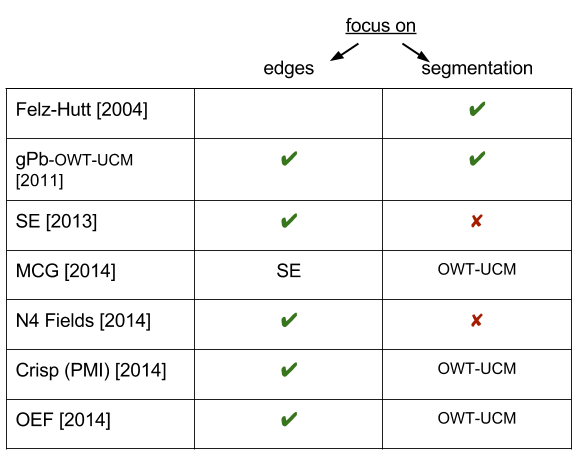
\includegraphics[width=0.7\textwidth]{images/related_work_table.png}
\caption[Related work: state of the art]{Review of the state-of-the-art methods for edge detection and segmentation.}
\label{fig:related_work_table}
\end{figure}

\section{Goal}
Our objectives are  twofold:  first to provide a principled way of obtaining hierarchical image segmentation based on probabilistic edge detection results, and second, to explore ways to improve the quality of the so %thus 
obtained segmentation.

% a more principled approach to boundary-guided image segmentation. % analysis?
% \section{Outline}
% The rest of this work is structured as follows:



% \begin{itemize}
% \item Chapter~\ref{SpectRelax} starts the thesis with a brief introduction to balanced graph cuts and spectral relaxation techniques.
% Section~\ref{sec:ch2_clgrpart} shows that clustering can be seen as a graph partitioning problem. The minimum cut approach often yields useless results where clusters are highly unbalanced, hence
% the balanced graph cut criteria are described in Section~\ref{sec:ch2_balgrcut}.  To solve the NP-hard balanced graph cut problem
% the relaxation methods are applied. Section~\ref{sec:ch2_spectclus} presents the standard spectral clustering approach, which is known to be loose.
% The tight relaxation, called 1-spectral clustering, is described in Section~\ref{sec:ch2_1spectclus}. 
% Section~\ref{ch2:disc} concludes the chapter and discusses the relevance of proposed methods to video segmentation.
% \item Chapter~\ref{chapter3} gives an overview of the video segmentation framework and provides the analysis of low-level features.
% Section~\ref{sec:ch3_framework} introduces the proposed video segmentation model, which employs a two-step approach:
% a graph is constructed on pre-computed superpixels and then a spectral clustering technique is applied. 
% %In graph-based algorithms, in order to produce high-quality segmentation results powerful superpixel similarity measures must be defined.
% Section~\ref{sec:ch3_affinities} gives a description of the graph affinities used in this work.
% To evaluate video segmentation performance and analyze the features of the proposed model we chose the Berkeley motion segmentation dataset, which is presented in Section~\ref{sec:ch3_dataset}.  
% The examination of the quality of the low-level video features is reported in Section~\ref{sec:ch3_aff} and the results are discussed in Section~\ref{ch3:disc}.
% \item Chapter~\ref{Chapter4} provides an experimental comparison of spectral relaxations and analyzes the effects of different balanced graph cuts applied to video segmentation. 
% We start with a brief recap of the main theoretical aspects of 1-norm and 2-norm relaxations in Section~\ref{ch4:recap}.
% Section~\ref{ch4:bench} presents the evaluation benchmark for video segmentation.
% Section~\ref{sec:ch4_1sc_vs_sc} shows the comparison of the performance of spectral clustering and 1-spectral clustering with different balanced graph cut objectives in the task of video segmentation. 
% In order to explore further the balanced cut criteria and the quality of the solutions obtained from the relaxation techniques, we tried to find a better partition by a trivial greedy search optimizing different balanced graph cut functions and see if the ground truth corresponds
% with the minimum cut criterion. The results of the experiments are reported in Section~\ref{sec:ch4_GTexp}.
% Section~\ref{ch4:disc} gives the discussion of the obtained results.
% \item In Chapter~\ref{Chapter5} a methodology for discriminative learning of must-link constraints and their incorporation in the video segmentation framework are proposed.
% Section~\ref{sec:ch5_cosc} shows a way of integrating prior information in the form of must-link constraints into spectral clustering while preserving all the
% balanced graph cuts.
% Section~\ref{sec:llf} presents evaluation of the low-level features as must-link constraints and the connections in the graph based on the ground truth.
% In Section~\ref{sec:ch4_ML} we propose to learn must-links with Random Forest from the affinities.
% We show that even a naive learning approach on the restricted feature space improves video segmentation performance for both relaxations: spectral clustering and 1 spectral clustering. 
% The proposed model is compared to state-of-the-art methods.
% Section~\ref{ch5:disc} discusses the achieved results.
% \item Chapter~\ref{Chapter6} concludes the thesis summarizing all the results of our work and proposing directions for possible improvements.
% \end{itemize}
